\documentclass[11pt,a4paper]{article}
\usepackage[T1]{fontenc}
\usepackage[margin=2.3cm]{geometry}
\usepackage{amsmath,amssymb}
\usepackage{graphicx}
\usepackage[dvipsnames]{xcolor}
\usepackage{enumitem}
\usepackage[colorlinks=true,linkcolor=blue,urlcolor=blue]{hyperref}
\setlength{\parskip}{0.6em}
\setlength{\parindent}{0pt}
\begin{document}

\begin{center}{\LARGE\bfseries openregression}\\[0.4em]{\large Predict crop yield from rainfall, and learn to catch a model that only memorised the past.}\\[0.2em]\small PAN IIT OSS explainer \textbullet{} higher secondary to advanced undergraduate (levels 4-6)\end{center}

\section*{Why this exists}
Regression is the art of predicting a number from other numbers and saying how much to trust the prediction. This explainer follows a farm example from a line through ten dots to a model that is audited for overfitting, using only a few lines of linear algebra.

\section*{The end goal}
Predict crop yield with regression and spot overfitting. The end goal is to predict crop yield with regression and to spot overfitting, the core skill of supervised learning. The same ideas (least squares, validation, regularisation, intervals) underlie forecasting, calibration and machine learning at every scale.

\section*{How the three sessions build up}
\begin{enumerate}[nosep]
\item \textbf{Session 1: The line that misses least} (Level 1, conceptual interactive model, 60 min).
\item \textbf{Session 2: Least squares, R squared and honest uncertainty} (Level 2, mathematical engineering model, 80 min).
\item \textbf{Session 3: Overfitting, ridge and honest validation} (Level 3, simulation and validation, 90 min).
\end{enumerate}

\section{Session 1: The line that misses least}

\subsection*{A. Real-world problem}
A farmer has ten seasons of records: how much rain fell and how much grain the field gave. Next season's rain forecast is known. What yield should the farmer expect? Drawing a line through the dots and reading off the answer is the idea of regression. But a hundred different lines can be drawn through the same dots. Which one is fair to call best? (All data here are made up for teaching; this is not advice about real farming.)

\subsection*{B. Concept and theory}
A straight line predicts yield from rain: prediction = a + b x. The intercept a is the yield predicted for zero rain; the slope b is the extra yield for each extra 100 mm. A residual is the observed yield minus the prediction, so it is the vertical distance from the dot to the line (positive if the dot is above). Adding the residuals would let misses above and below cancel, so we square them first. The total of the squares is the sum of squared residuals, SSE. The best line, called the least-squares line, has the smallest SSE. For ten farm seasons it is yield = 0.887 + 0.344 x, with SSE 0.378 (t/ha)\textasciicircum{}2.

\begin{itemize}[nosep]
\item x: rainfall in a season (hundreds of mm, so 3.0 means 300 mm) (100 mm)
\item y: grain yield (t/ha)
\item a: intercept of the line (t/ha)
\item b: slope of the line (t/ha per 100 mm)
\item e: residual = y - (a + b x) (t/ha)
\item SSE: sum of squared residuals ((t/ha)\textasciicircum{}2)
\end{itemize}

\begin{equation*}
\hat y = a + b\,x,\qquad e_i = y_i-(a+b\,x_i)
\end{equation*}

\begin{equation*}
\mathrm{SSE}(a,b)=\sum_{i=1}^{n} e_i^{2}
\end{equation*}

\begin{equation*}
b=\frac{\sum (x_i-\bar x)(y_i-\bar y)}{\sum (x_i-\bar x)^2},\qquad a=\bar y-b\,\bar x
\end{equation*}

\begin{center}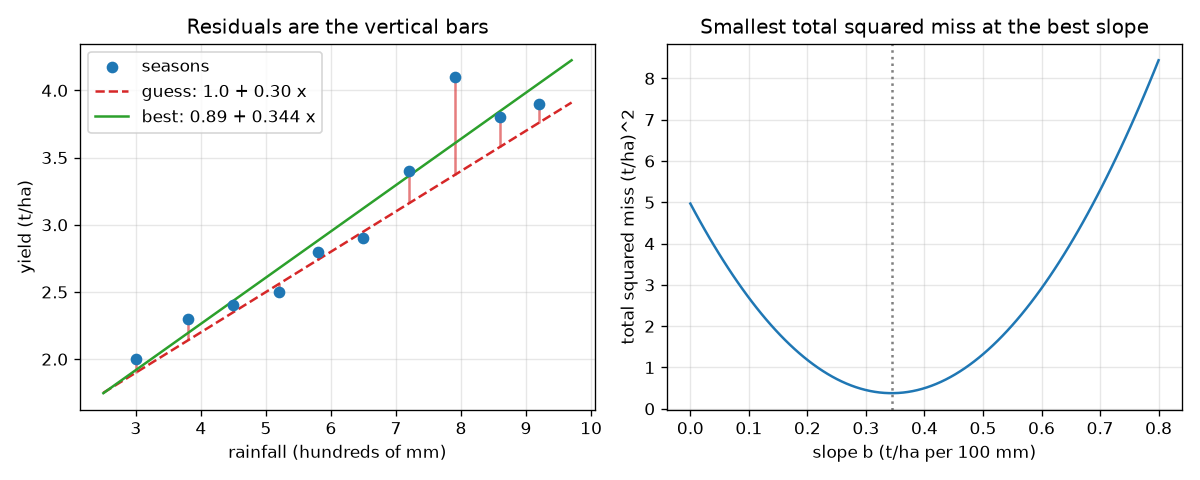
\includegraphics[width=0.85\linewidth]{figures/s01_dots_and_line.png}\\\small Ten seasons, a guess line with its residual bars, the best line, and the bowl of total squared miss against slope.\end{center}

\subsection*{E. Worked example}
Three dots (rain, yield) are (1, 2), (2, 2) and (3, 5). Find the least-squares line and its total squared miss by hand.
\begin{enumerate}[nosep]
\item Means: x-bar = (1 + 2 + 3) / 3 = 2 and y-bar = (2 + 2 + 5) / 3 = 3.
\item Sum of (x - 2)(y - 3) = (-1)(-1) + (0)(-1) + (1)(2) = 1 + 0 + 2 = 3. Sum of (x - 2)\textasciicircum{}2 = 1 + 0 + 1 = 2.
\item Slope b = 3 / 2 = 1.5. Intercept a = 3 - 1.5 * 2 = 0.
\item Predictions: 1.5, 3.0, 4.5. Residuals: 2 - 1.5 = 0.5, 2 - 3 = -1, 5 - 4.5 = 0.5.
\item SSE = 0.25 + 1 + 0.25 = 1.5. Check: the residuals add up to 0.5 - 1 + 0.5 = 0.
\end{enumerate}
\textbf{Answer.} The line is y = 0 + 1.5 x with residuals 0.5, -1 and 0.5 and total squared miss 1.5.

\subsection*{F. Questions}
\begin{enumerate}[nosep]
\item \textbf{Conceptual.} Why do we square the residuals instead of just adding them up? What would happen to the line 'sum of residuals = 0' test?
\item \textbf{Numerical.} Find the least-squares line for the dots (0, 2), (1, 1) and (2, 6), and its total squared miss.
\item \textbf{Graph and simulation interpretation.} In the bowl view, at which slope is the green curve lowest, and what is its value there? Why is the blue curve never below the green one?
\item \textbf{Design and optimisation challenge.} Design: using the best line of the farm data, how much rain gives an expected yield of 3.5 t/ha? Is the answer inside the range of the data? What should you worry about?
\end{enumerate}

\section{Session 2: Least squares, R squared and honest uncertainty}

\subsection*{A. Real-world problem}
A farm adviser says: 'to reach 3.5 tonnes per hectare you need about 716 mm of rain'. A good adviser adds how sure she is. How much rain makes the target likely rather than just average? And can she trust the line when the forecast is 1000 mm, wetter than any season on record? This session turns the best line into a calculation with an honest margin of error. All data are synthetic, generated with known coefficients so that we can check our answers.

\subsection*{B. Concept and theory}
Stack the data as y = X beta: each row of X is (1, x) and beta = (a, b). The total squared miss is S(beta) = (y - X beta)\textasciicircum{}T (y - X beta). Setting its derivative to zero gives -2 X\textasciicircum{}T (y - X beta) = 0, the normal equations (X\textasciicircum{}T X) beta = X\textasciicircum{}T y. They say the residual vector is perpendicular to every column of X. R squared = 1 - SS\_res / SS\_tot is the fraction of the variation of y about its mean that the line explains; for one input it equals the square of the correlation. It does not prove the model is right: if the residuals show a pattern (a curve, a funnel), the model is wrong however large R squared is. With two inputs (rain r and fertiliser f) X has three columns and the same equations hold. A prediction interval for one new season at x0 is yhat0 +- t s sqrt(1 + 1/n + (x0 - x-bar)\textasciicircum{}2 / Sxx), where s\textasciicircum{}2 = SS\_res / (n - 2) and t is the Student t quantile with n - 2 degrees of freedom. The '1' inside the root is the season's own noise; the other terms are uncertainty in the line, which grows with the distance from x-bar. Extrapolating beyond the data is dangerous because the formula assumes the line still holds.

\begin{itemize}[nosep]
\item X: design matrix: a column of ones, then the inputs (no unit)
\item beta: vector of coefficients (a, b, ...) (t/ha and t/ha per input unit)
\item SS\_res: sum of squared residuals ((t/ha)\textasciicircum{}2)
\item SS\_tot: sum of (y - y-bar)\textasciicircum{}2 ((t/ha)\textasciicircum{}2)
\item R\textasciicircum{}2: fraction of variation explained (no unit)
\item s: residual standard deviation, sqrt(SS\_res / (n - p)) (t/ha)
\item t: Student t quantile (0.975, n - 2 degrees of freedom) (no unit)
\item Sxx: sum of (x - x-bar)\textasciicircum{}2 ((100 mm)\textasciicircum{}2)
\end{itemize}

\begin{equation*}
(X^{\mathsf T}X)\,\beta = X^{\mathsf T}y\quad\Longleftrightarrow\quad X^{\mathsf T}(y-X\beta)=0
\end{equation*}

\begin{equation*}
R^2 = 1-\frac{\mathrm{SS}_{\mathrm{res}}}{\mathrm{SS}_{\mathrm{tot}}},\qquad \mathrm{SS}_{\mathrm{tot}}=\sum (y_i-\bar y)^2
\end{equation*}

\begin{equation*}
\hat y_0 \pm t_{0.975,\,n-2}\; s\,\sqrt{1+\frac{1}{n}+\frac{(x_0-\bar x)^2}{S_{xx}}}
\end{equation*}

\begin{equation*}
\widehat{\mathrm{SE}}(\hat\beta_j)=\sqrt{s^2\,[(X^{\mathsf T}X)^{-1}]_{jj}}
\end{equation*}

\begin{center}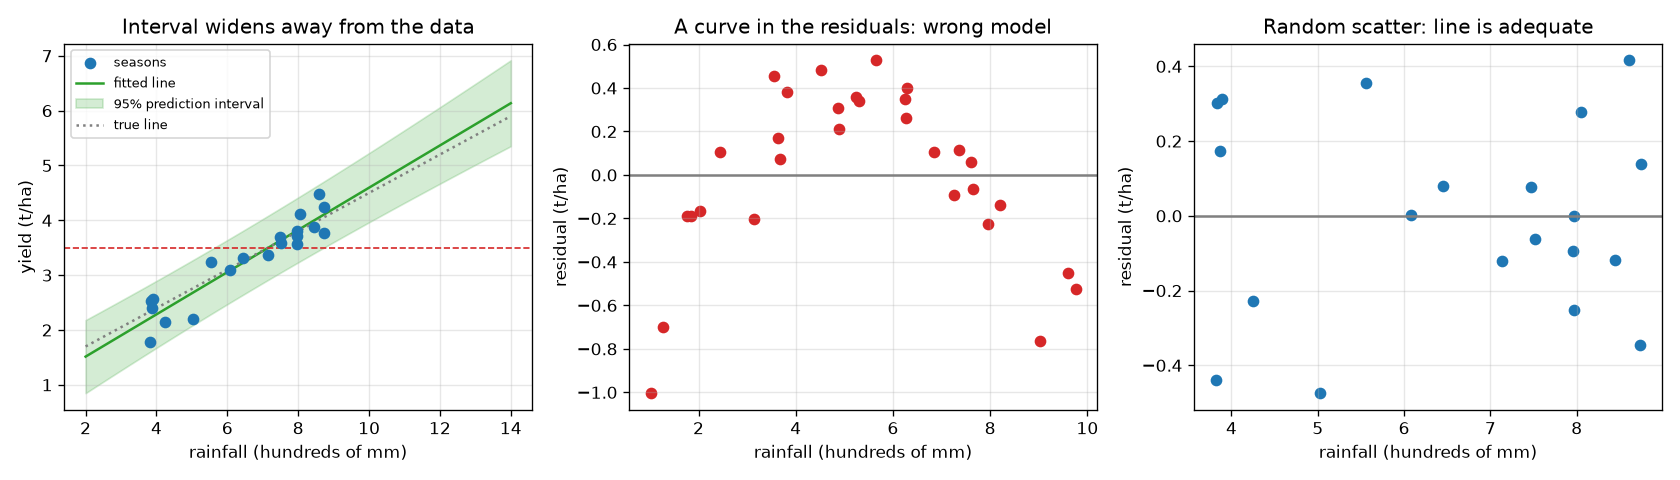
\includegraphics[width=0.85\linewidth]{figures/s02_residuals_and_interval.png}\\\small Left: fitted line with a 95 percent prediction band and the 3.5 t/ha target. Middle: arch-shaped residuals of a line through curved data. Right: shapeless residuals of a line through straight data.\end{center}

\subsection*{E. Worked example}
For the dots (1, 2), (2, 2), (3, 5) compute R squared by hand, then predict the yield at x = 4.
\begin{enumerate}[nosep]
\item From Session 1 the line is y = 0 + 1.5 x with residuals 0.5, -1, 0.5, so SS\_res = 1.5.
\item The mean of y is 3, so SS\_tot = (2 - 3)\textasciicircum{}2 + (2 - 3)\textasciicircum{}2 + (5 - 3)\textasciicircum{}2 = 1 + 1 + 4 = 6.
\item R squared = 1 - 1.5 / 6 = 0.75.
\item Check with the correlation: r = Sxy / sqrt(Sxx Syy) = 3 / sqrt(2 * 6) = 0.866, and r\textasciicircum{}2 = 0.75.
\item Prediction at x = 4: 0 + 1.5 * 4 = 6.0. This is extrapolation (the data stop at 3), so it deserves little trust.
\end{enumerate}
\textbf{Answer.} R squared = 0.75 (75 percent of the variation explained) and the prediction at x = 4 is 6.0, an extrapolation.

\subsection*{F. Questions}
\begin{enumerate}[nosep]
\item \textbf{Conceptual.} A line fitted to curved data has R squared 0.837. Is it a good model? What does the residual plot show, and what would you do?
\item \textbf{Numerical.} For the dots (1, 2), (2, 2), (3, 5) the best line is y = 1.5 x. Show that the normal equations hold, i.e. that X\textasciicircum{}T e = 0 for the residuals e = (0.5, -1, 0.5).
\item \textbf{Graph and simulation interpretation.} In the app (noise 0.30 t/ha, 20 seasons) the band is narrowest at 600 mm. What is the half-width there, and what is it at 1100 mm? Why is it larger?
\item \textbf{Design and optimisation challenge.} Design: with 20 farm seasons, how much rain is needed for a 3.5 t/ha yield on average, and how much so that the lower end of the 95 percent prediction interval reaches 3.5 t/ha? Comment on the trade-off.
\end{enumerate}

\section{Session 3: Overfitting, ridge and honest validation}

\subsection*{A. Real-world problem}
A model with enough knobs can pass through every training point and still predict next season badly. Nothing looks wrong on the data it was built from, which is exactly why overfitting is dangerous. This session measures the effect, tames it with ridge regression, chooses settings with cross-validation instead of wishful thinking, and then meets three traps: wrong data points, a hidden variable that makes two things look connected (ice-cream sales and drownings), and two inputs that are almost copies of each other. It ends with a complete audit of a yield model. This is general education about modelling on synthetic data, not agronomic advice.

\subsection*{B. Concept and theory}
A degree-d polynomial has d + 1 coefficients. Training error (RMSE, in t/ha) can only fall as d grows. Test error, measured on fresh data, falls and then rises: a U shape. The total expected error splits into noise (which nobody can remove), squared bias (the model cannot bend enough) and variance (the fit changes a lot from one data set to another). Flexible models have low bias and high variance. Ridge regression shrinks the coefficients by adding lambda times their squared size to the loss; on standardised features (subtract the mean, divide by the standard deviation) the solution is beta = (X\textasciicircum{}T X + lambda I)\textasciicircum{}-1 X\textasciicircum{}T y, and lambda = 0 gives ordinary least squares. We choose lambda or the degree by k-fold cross-validation: split the training seasons into k parts, train on k - 1, score on the rest, rotate and average. Least squares is damaged by outliers; the Theil-Sen line (median of pairwise slopes) and the Huber line (iteratively reweighted least squares) resist them. A confounder (temperature) can create a correlation between two quantities that do not influence each other; the partial correlation, after removing the confounder's linear effect from both, shows it. If two inputs are nearly identical the condition number of X\textasciicircum{}T X explodes: the coefficients become wild (huge variance) while predictions that use them together stay fine. Because the data are synthetic we can check the fits against the truth: slope +- 1.96 standard errors should hold the true slope in about 95 percent of repeats, and the standard error falls like 1 / sqrt(n).

\begin{itemize}[nosep]
\item d: polynomial degree (no unit)
\item lambda: ridge penalty strength (no unit (features standardised))
\item RMSE: root mean squared error = sqrt(mean of squared misses) (t/ha)
\item k: number of cross-validation folds (no unit)
\item z: scaled rainfall in [-1, 1] (no unit)
\item cond: condition number of X\textasciicircum{}T X (largest / smallest eigenvalue) (no unit)
\item rho(A,B \textbar{} T): partial correlation of A and B given T (no unit)
\end{itemize}

\begin{equation*}
\hat\beta_{\mathrm{ridge}}=(X^{\mathsf T}X+\lambda I)^{-1}X^{\mathsf T}y
\end{equation*}

\begin{equation*}
\mathbb E\big[(\hat f(z_0)-y_0)^2\big]=\sigma^2+\mathrm{bias}^2+\mathrm{variance}
\end{equation*}

\begin{equation*}
\mathrm{CV}_k=\frac1k\sum_{j=1}^{k}\mathrm{RMSE}_j\ \text{ (RMSE on fold } j \text{ after training on the others)}
\end{equation*}

\begin{equation*}
\rho_{AB\cdot T}=\mathrm{corr}\big(A-\hat A(T),\ B-\hat B(T)\big)
\end{equation*}

\begin{equation*}
\mathrm{SE}(\hat b)=\frac{\sigma}{\sqrt{S_{xx}}}
\end{equation*}

\begin{center}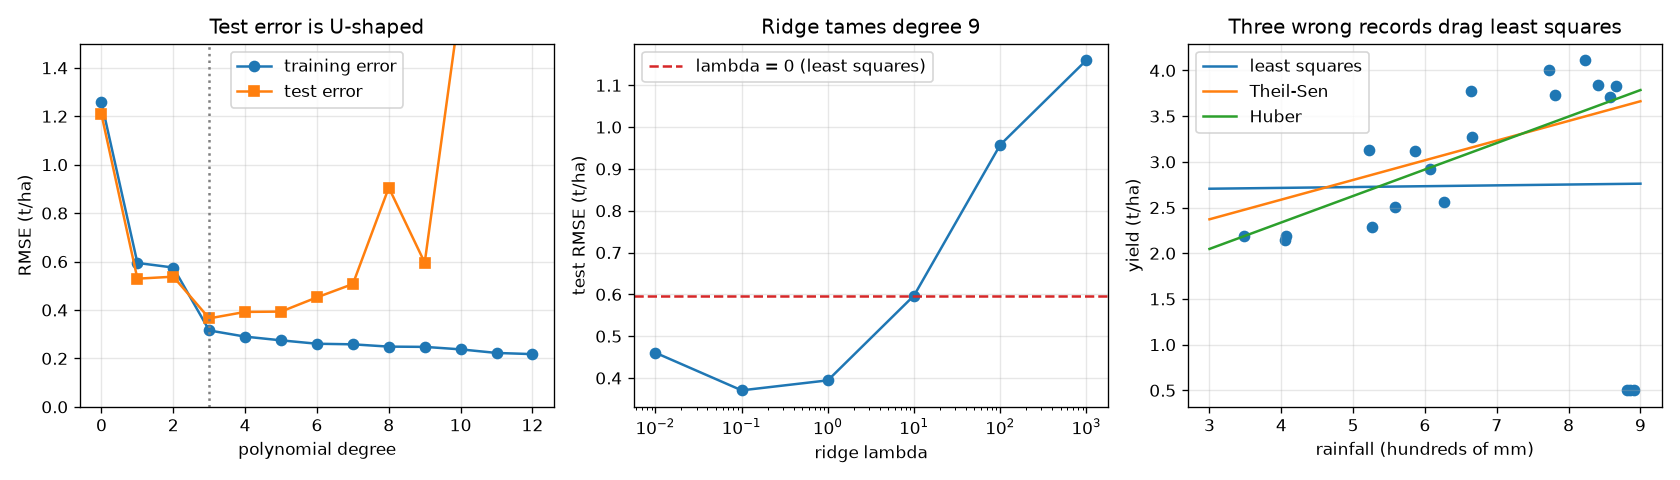
\includegraphics[width=0.85\linewidth]{figures/s03_overfit_ridge_robust.png}\\\small Left: training and test error against degree. Middle: ridge test error against lambda. Right: robust lines against least squares when three records are wrong.\end{center}

\subsection*{E. Worked example}
Three points x = -1, 0, 1 with y = 0, 1, 5. Compute the ridge slope by hand for lambda = 0 and lambda = 3 (standardise x first), and convert back to the original units.
\begin{enumerate}[nosep]
\item x-bar = 0 and the standard deviation (dividing by n) is sqrt(2/3) = 0.8165, so the standardised values are about -1.2247, 0, 1.2247.
\item y-bar = 2, so the centred y are -2, -1, 3. X\textasciicircum{}T X = 3 (sum of squares of standardised x) and X\textasciicircum{}T y = (-1.2247)(-2) + (1.2247)(3) = 6.1237.
\item Ridge slope = 6.1237 / (3 + lambda). For lambda = 0 this is 2.0412; for lambda = 3 it is 1.0206, exactly half.
\item Back to original units divide by 0.8165: 2.5 for lambda = 0 (the ordinary slope Sxy / Sxx = 5 / 2) and 1.25 for lambda = 3.
\end{enumerate}
\textbf{Answer.} Ridge slope 2.5 at lambda = 0 (least squares) and 1.25 at lambda = 3: the penalty multiplies the slope by 3 / (3 + lambda).

\subsection*{F. Questions}
\begin{enumerate}[nosep]
\item \textbf{Conceptual.} A colleague picks the polynomial degree with the smallest training error and reports it. Why is that wrong, and what should be done instead?
\item \textbf{Numerical.} For the three points x = -1, 0, 1 with y = 0, 1, 5, find the ridge slope in original units for lambda = 6.
\item \textbf{Graph and simulation interpretation.} In the app, at degree 9, compare the expected test error at log10 lambda = -4 and at -1. What does each tell you about the fit?
\item \textbf{Design and optimisation challenge.} Design: for the farm data set of the mini-project, you can deploy the mean only, rain only, the three inputs, or the too-flexible model. Choose by cross-validation and give the forecast for 550 mm, 60 kg/ha, 25 degrees C with its interval. What do you tell the farmer about it?
\end{enumerate}

\section{Real-world mini-project}
\textbf{Build and audit a yield model for next season.} A synthetic farm has 60 seasons of data: rain (hundreds of mm), fertiliser (10 kg/ha units) and mean temperature (degrees C). Use \texttt{farm\_dataset}, fit yield on the three inputs by least squares, audit it, and forecast next season (550 mm of rain, 60 kg/ha, 25 degrees C). The audit must compare four models by 6-fold cross-validation: the mean only, rain only, the three inputs, and a too-flexible model with all squares and products. This is a teaching exercise on invented data, not agronomic advice.

\section{The path ahead}
\begin{enumerate}[nosep]
\item \textbf{Session 4: Intervals when the noise grows.} A prediction interval that estimates the noise level as a function of rain.
\item \textbf{Session 5: A smooth model without choosing a degree.} A smoother that replaces the polynomial in the degree-versus-error experiment.
\item \textbf{Session 6: Models that switch features off.} A lasso solver by coordinate descent, written from the roadmap.
\item \textbf{Session 7: Planning for a bad season.} A line fitted by minimising the pinball loss.
\end{enumerate}

\section{Answers and hints}

\subsection*{Session 1}
\begin{enumerate}[nosep]
\item \textbf{Conceptual.} Hint: Think of one dot far above the line and one far below. Solution: Residuals above and below the line have opposite signs and cancel, so the plain sum can be zero for a terrible line: any line through the point (x-bar, y-bar) has residuals that add to zero, whatever its slope. Squaring makes every miss positive and makes a large miss count more than several small ones, so only a line that is close to all the dots gets a small total.
\item \textbf{Numerical.} Hint: x-bar = 1, y-bar = 3. Use b = sum((x - x-bar)(y - y-bar)) / sum((x - x-bar)\textasciicircum{}2). Solution: Sum of (x - 1)(y - 3) = (-1)(-1) + 0 + (1)(3) = 4 and sum of (x - 1)\textasciicircum{}2 = 2, so b = 2 and a = 3 - 2 = 1. Predictions 1, 3, 5 give residuals 1, -2, 1 and SSE = 1 + 4 + 1 = 6 (units t/ha squared if the numbers are yields).
\item \textbf{Graph and simulation interpretation.} Hint: The green curve uses the best intercept for every slope. Solution: The green curve is lowest at slope 0.344 t/ha per 100 mm, where it equals 0.378 (t/ha)\textasciicircum{}2, the best possible total. The blue curve uses your own intercept, which is not the best for most slopes, so it can touch the green curve but never go below it.
\item \textbf{Design and optimisation challenge.} Hint: Solve 3.5 = 0.887 + 0.344 x for x. Solution: x = (3.5 - 0.887) / 0.344 = 7.59 hundreds of mm, that is about 759 mm. The data cover 300 to 920 mm, so this is interpolation, which is safer than extrapolation. But it is only the expected yield: single seasons scatter around the line (Session 2 puts a number on that), so a season with that rain can easily give less than 3.5 t/ha.
\end{enumerate}

\subsection*{Session 2}
\begin{enumerate}[nosep]
\item \textbf{Conceptual.} Hint: R squared measures how much variation is explained, not whether the shape is right. Solution: R squared of 0.837 is high, but the residuals form an arch (the correlation of the residuals with (x - x-bar)\textasciicircum{}2 is -0.90): negative at both ends and positive in the middle. A pattern in the residuals means the straight line is the wrong shape. We should add a curved term or use a saturating model, not trust the line for forecasts.
\item \textbf{Numerical.} Hint: The columns of X are (1, 1, 1) and (1, 2, 3). Solution: Column of ones: 0.5 - 1 + 0.5 = 0. Column of x: 1 * 0.5 + 2 * (-1) + 3 * 0.5 = 0.5 - 2 + 1.5 = 0. Both products vanish, so the residuals are perpendicular to both columns, which is exactly the normal equations.
\item \textbf{Graph and simulation interpretation.} Hint: Read the readout at x0 = 6 and at x0 = 11. Solution: At 600 mm the half-width is 0.65 t/ha (mostly the season's own noise) and at 1100 mm it is 0.76 t/ha, because the term (x0 - x-bar)\textasciicircum{}2 / Sxx grows with the distance from the mean rain: the slope's uncertainty is multiplied by a longer lever arm. The band flares like a bow tie around the centre of the data.
\item \textbf{Design and optimisation challenge.} Hint: Invert the line for the first part; for the second, find the smallest rain whose lower bound is at least 3.5. Solution: The line gives 716 mm (x = 7.16 in 100 mm) for the average. For the lower bound of the 95 percent interval to reach 3.5 t/ha we need 872 mm, an extra 156 mm, because we are asking not for the average season but for nearly every season. Both values lie inside the data range (up to 900 mm), so no extrapolation is needed. The trade-off: certainty costs rain (or irrigation); a farmer who accepts a 1-in-20 miss on the lower side pays less.
\end{enumerate}

\subsection*{Session 3}
\begin{enumerate}[nosep]
\item \textbf{Conceptual.} Hint: Compare the training error at degree 3 and degree 12. Solution: Training error can only go down as degree increases (0.22 t/ha at degree 12 against about 0.32 at degree 3), so choosing by training error always picks the most flexible model, which here has a test error of 5.1 t/ha. Choose by error on data the model has not seen: a separate test set or k-fold cross-validation.
\item \textbf{Numerical.} Hint: The slope is multiplied by 3 / (3 + lambda) compared with least squares (2.5). Solution: Factor = 3 / (3 + 6) = 1/3, so the slope is 2.5 / 3 = 0.833. The larger the penalty, the closer the slope gets to zero (and the prediction to the mean of y).
\item \textbf{Graph and simulation interpretation.} Hint: Read the readout and the fit view for both settings. Solution: At log10 lambda = -4 (practically least squares) the training error is 0.250 but the expected test error is 0.832 t/ha: the curve wiggles through the noise. At log10 lambda = -1 the training error rises to 0.291 but the expected test error falls to 0.357 t/ha, close to the noise floor of 0.30: ridge trades a little bias for much less variance.
\item \textbf{Design and optimisation challenge.} Hint: Use \texttt{farm\_audit} and \texttt{prediction\_interval\_multi}. Solution: 6-fold RMSE (t/ha): mean only 0.724, rain only 0.440, three inputs 0.343, too flexible 0.381. The three-input model wins and the flexible one is worse, a mild overfit. The forecast is 1.64 t/ha with a 95 percent prediction interval from 0.95 to 2.32 t/ha. The message: expect about 1.6 t/ha but a single season can plausibly land anywhere in that range; the model is built on synthetic data of one farm and says nothing about causes or about conditions outside the data.
\end{enumerate}

\section{How to join}
Read \texttt{CONTRIBUTING.md} in the repository, then pick an issue labelled \texttt{good first issue}. Repository: \url{https://github.com/KrunalPanchal1995/openregression}

\end{document}
